Further test were conducted by developing a new geometry. A scaled-down EG-CNTFET structure was designed with a channel and gate area reduced four times compared to the standard devices; the structure will be referred to as nEG-FET in the rest of the section. The nEG-FET was designed with a \SI{3}{\mm} $\times$ \SI{3}{\mm} gate and a \SI{1.5}{\mm} $\times$ \SI{1.5}{\mm} channel. The distance between the gate and the channel was scaled in proportion with the standard EG-CNTFET, amounting to \SI{0.75}{\mm}. The hypothesis to be tested was that fewer CNTs would take less time to reach stability, making subsequent sensing measurements faster, and would better maintain the stability achieved.

Photolithography and electrode deposition were carried out maintaining the same parameters as the previous two structures; on the other hand, the CNTs had to be optimized to obtain a working device. Indeed, it was assumed to adopt the same optimal working \rds{} range as for the larger structures, maintaining a target between \SI{1}{\kohm} and \SI{10}{\kohm}. The main change that occurred was the number of CNT layers required: it was found that \num{48} CNT layers were sufficient to achieve the previously-defined range, resulting in functional devices.

\begin{figure}
    \centering
    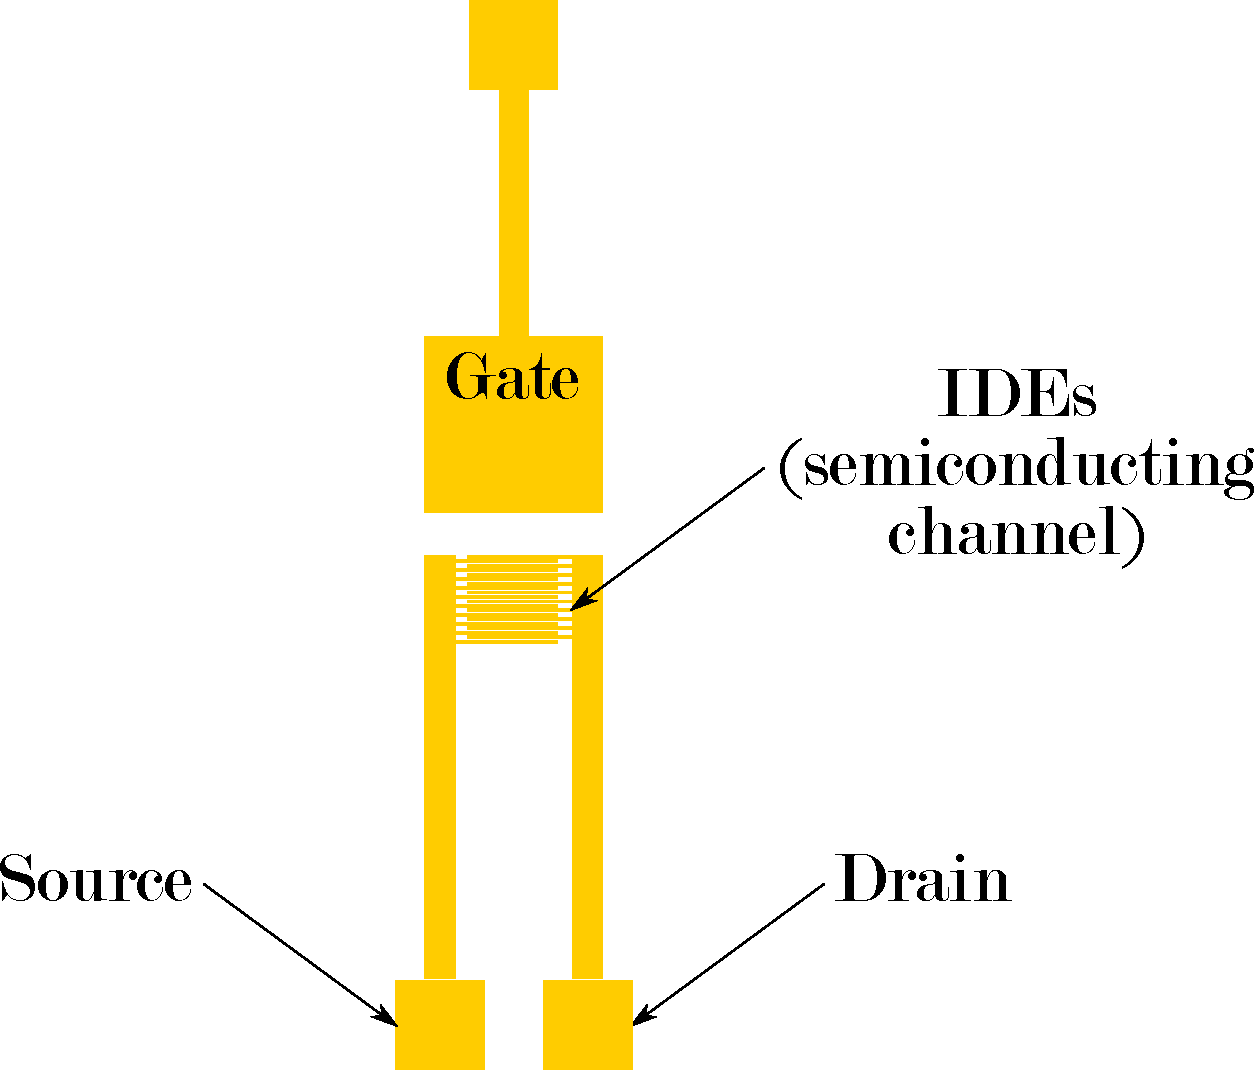
\includegraphics[width = 0.45\textwidth]{figures/chapter3/nEGFET/nEGFET_scheme.pdf}
    \caption{Illustration of an nEG-FET, with the channel area being four times smaller than the standard EG-FET and the sdEG-FET. In this configuration, the gate measures \SI{3}{\mm} $\times$ \SI{3}{\mm} and the channel has a side length of \SI{1.5}{\mm} $\times$ \SI{1.5}{\mm}. The distance between the gate and the channel is maintained in proportion to the standard geometry, being \SI{0.75}{\mm}.}
    \label{fig:nEGFET}
\end{figure}

\begin{figure}
    \centering
    \subfloat[Transfer characteristics of a device that did not stabilize]{
        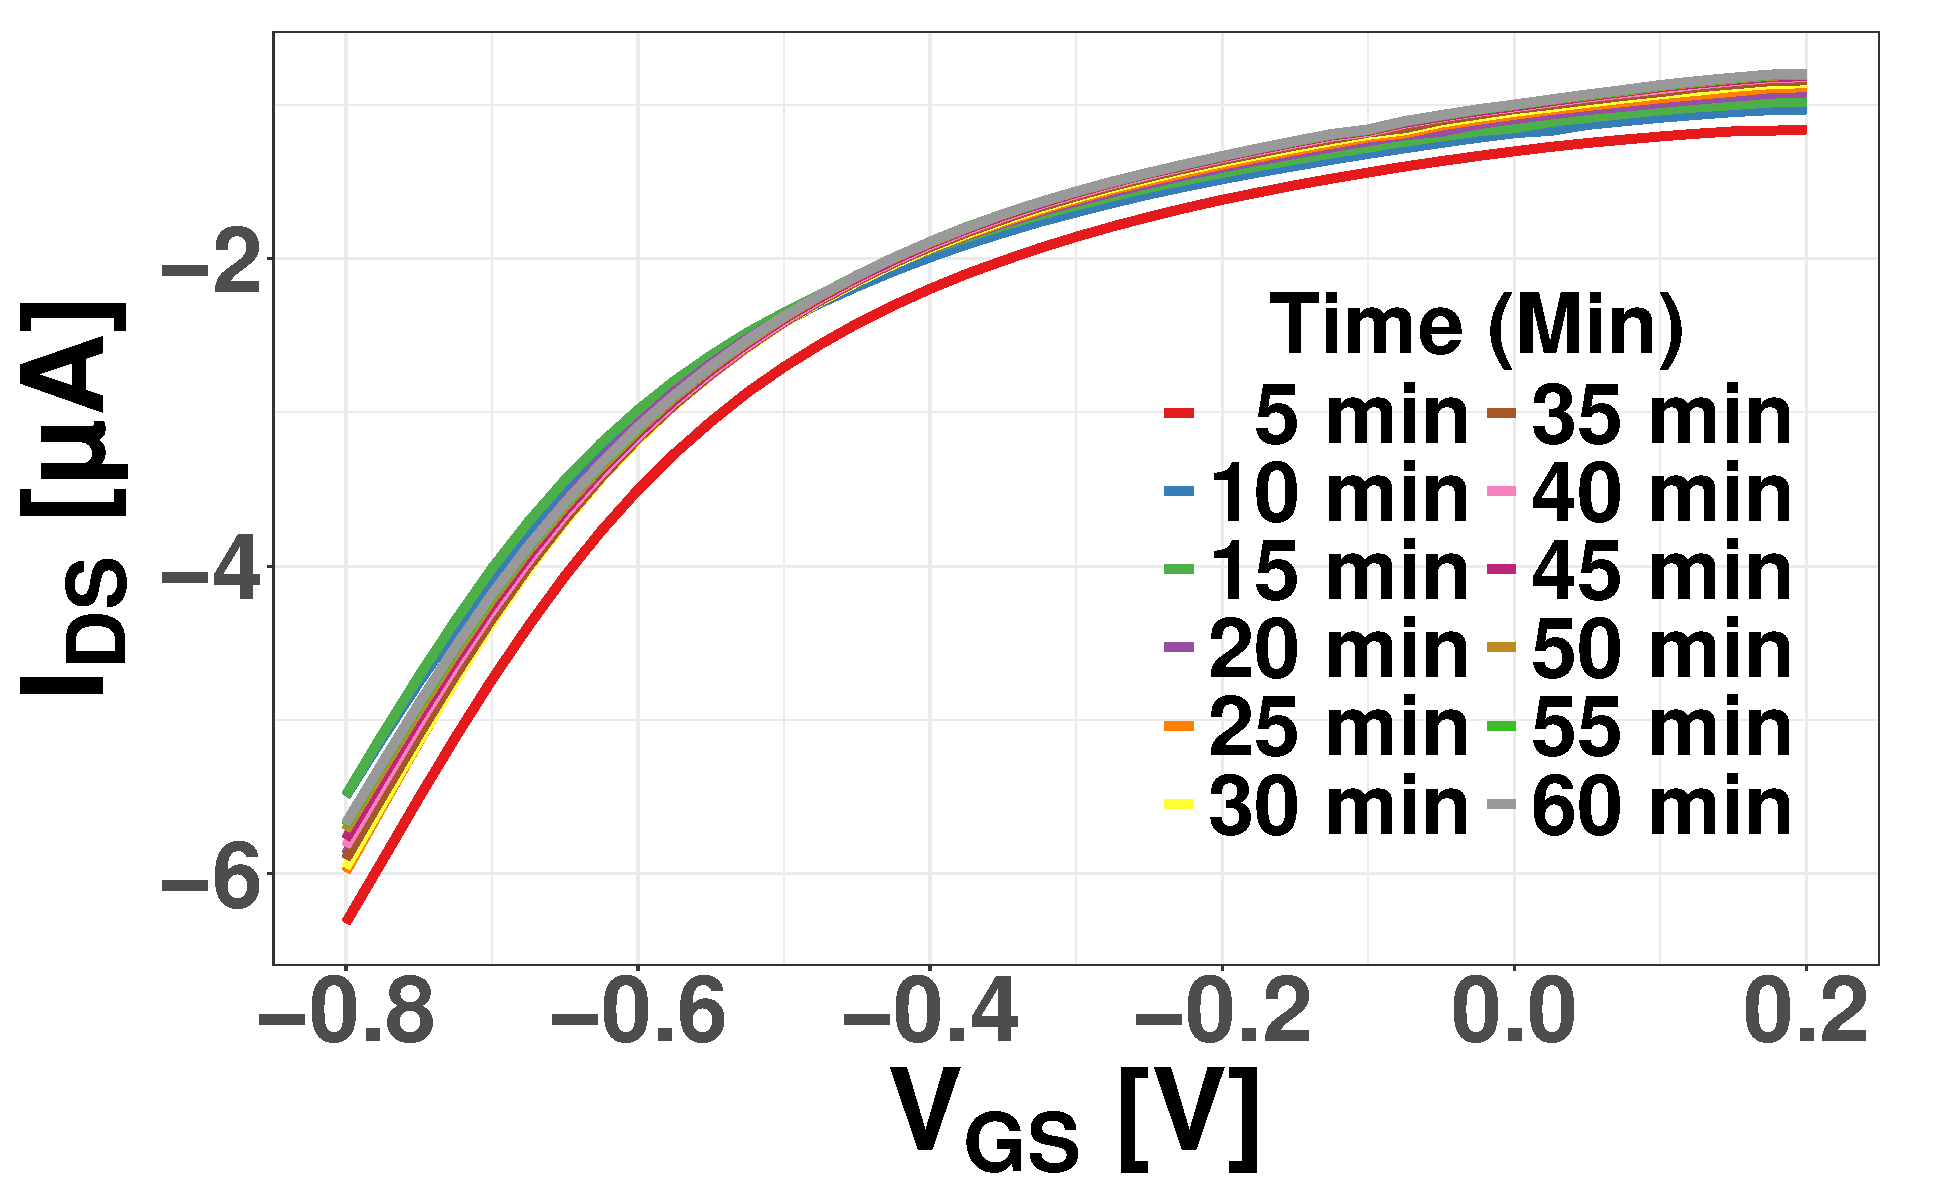
\includegraphics[width = 0.45\textwidth]{figures/chapter3/nEGFET/nTransfer_down.pdf}
        \label{fig:nTransferDown}
    }
    \hfill
    \subfloat[Normalized current of a device that did not stabilize]{
        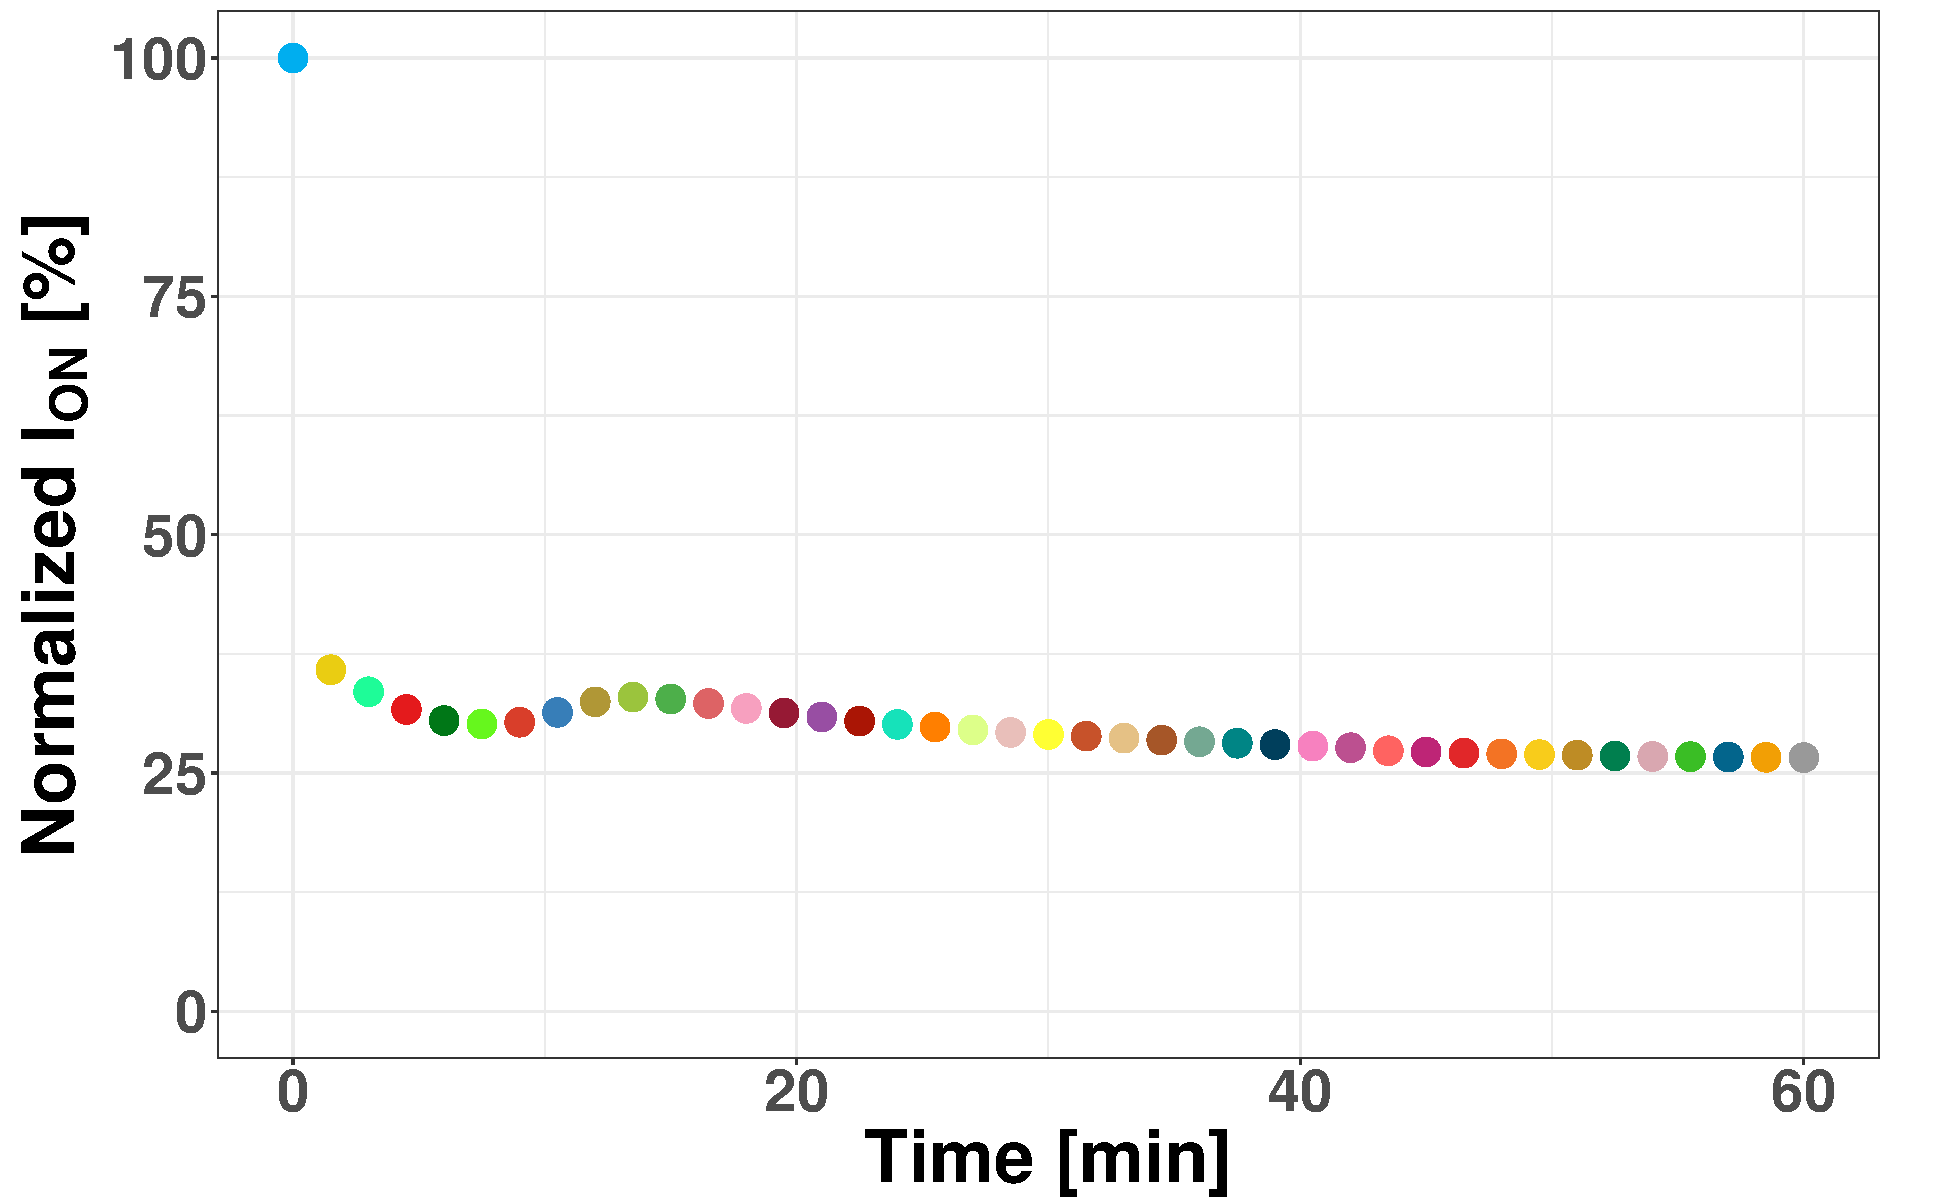
\includegraphics[width = 0.45\textwidth]{figures/chapter3/nEGFET/nNormalized_down.pdf}
        \label{fig:nNormalizedDown}
    } \\
    \subfloat[Transfer characteristics of a device that stabilized]{
        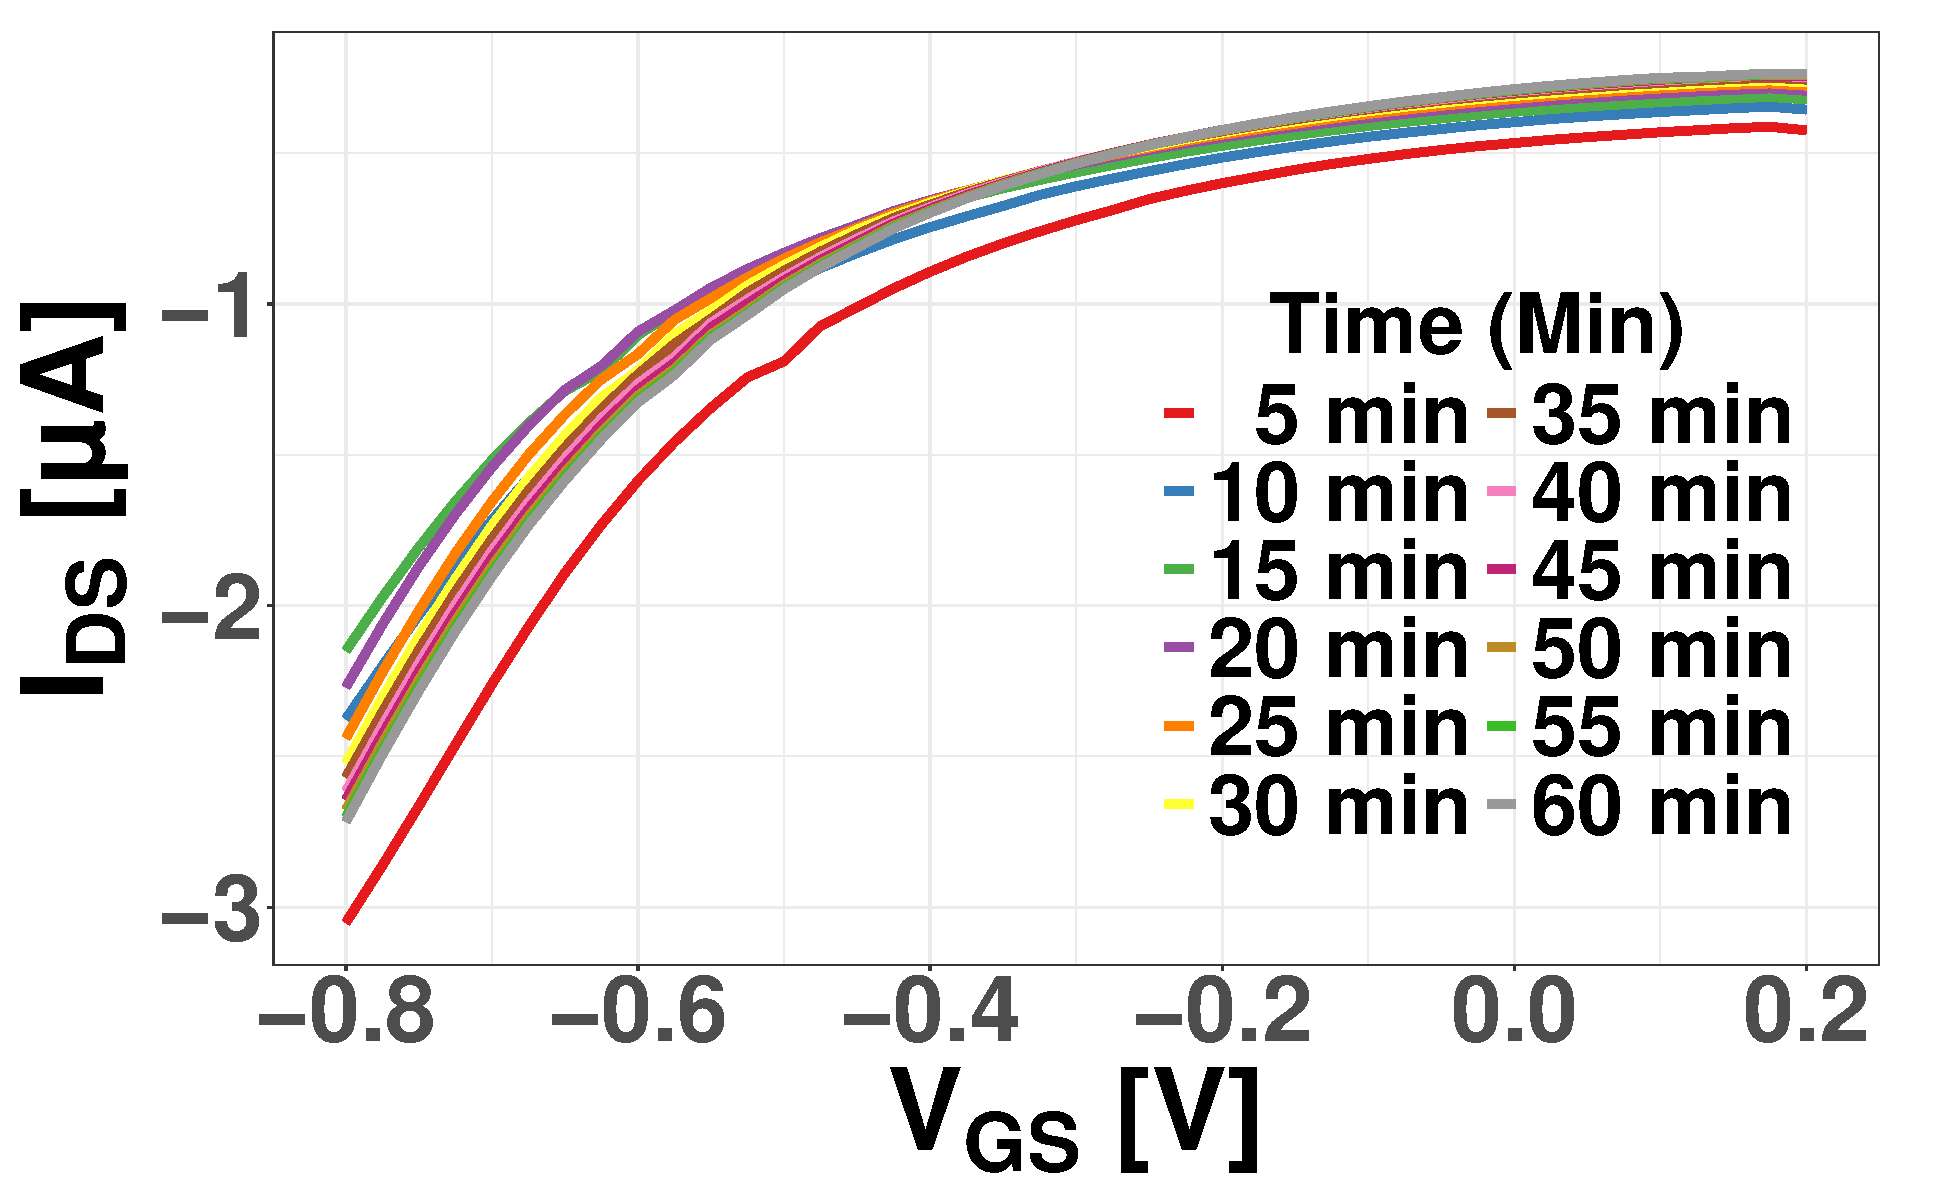
\includegraphics[width = 0.45\textwidth]{figures/chapter3/nEGFET/nTransfer_up.pdf}
        \label{fig:nTransferUp}
    }
    \hfill
    \subfloat[Normalized current of a device that stabilized]{
        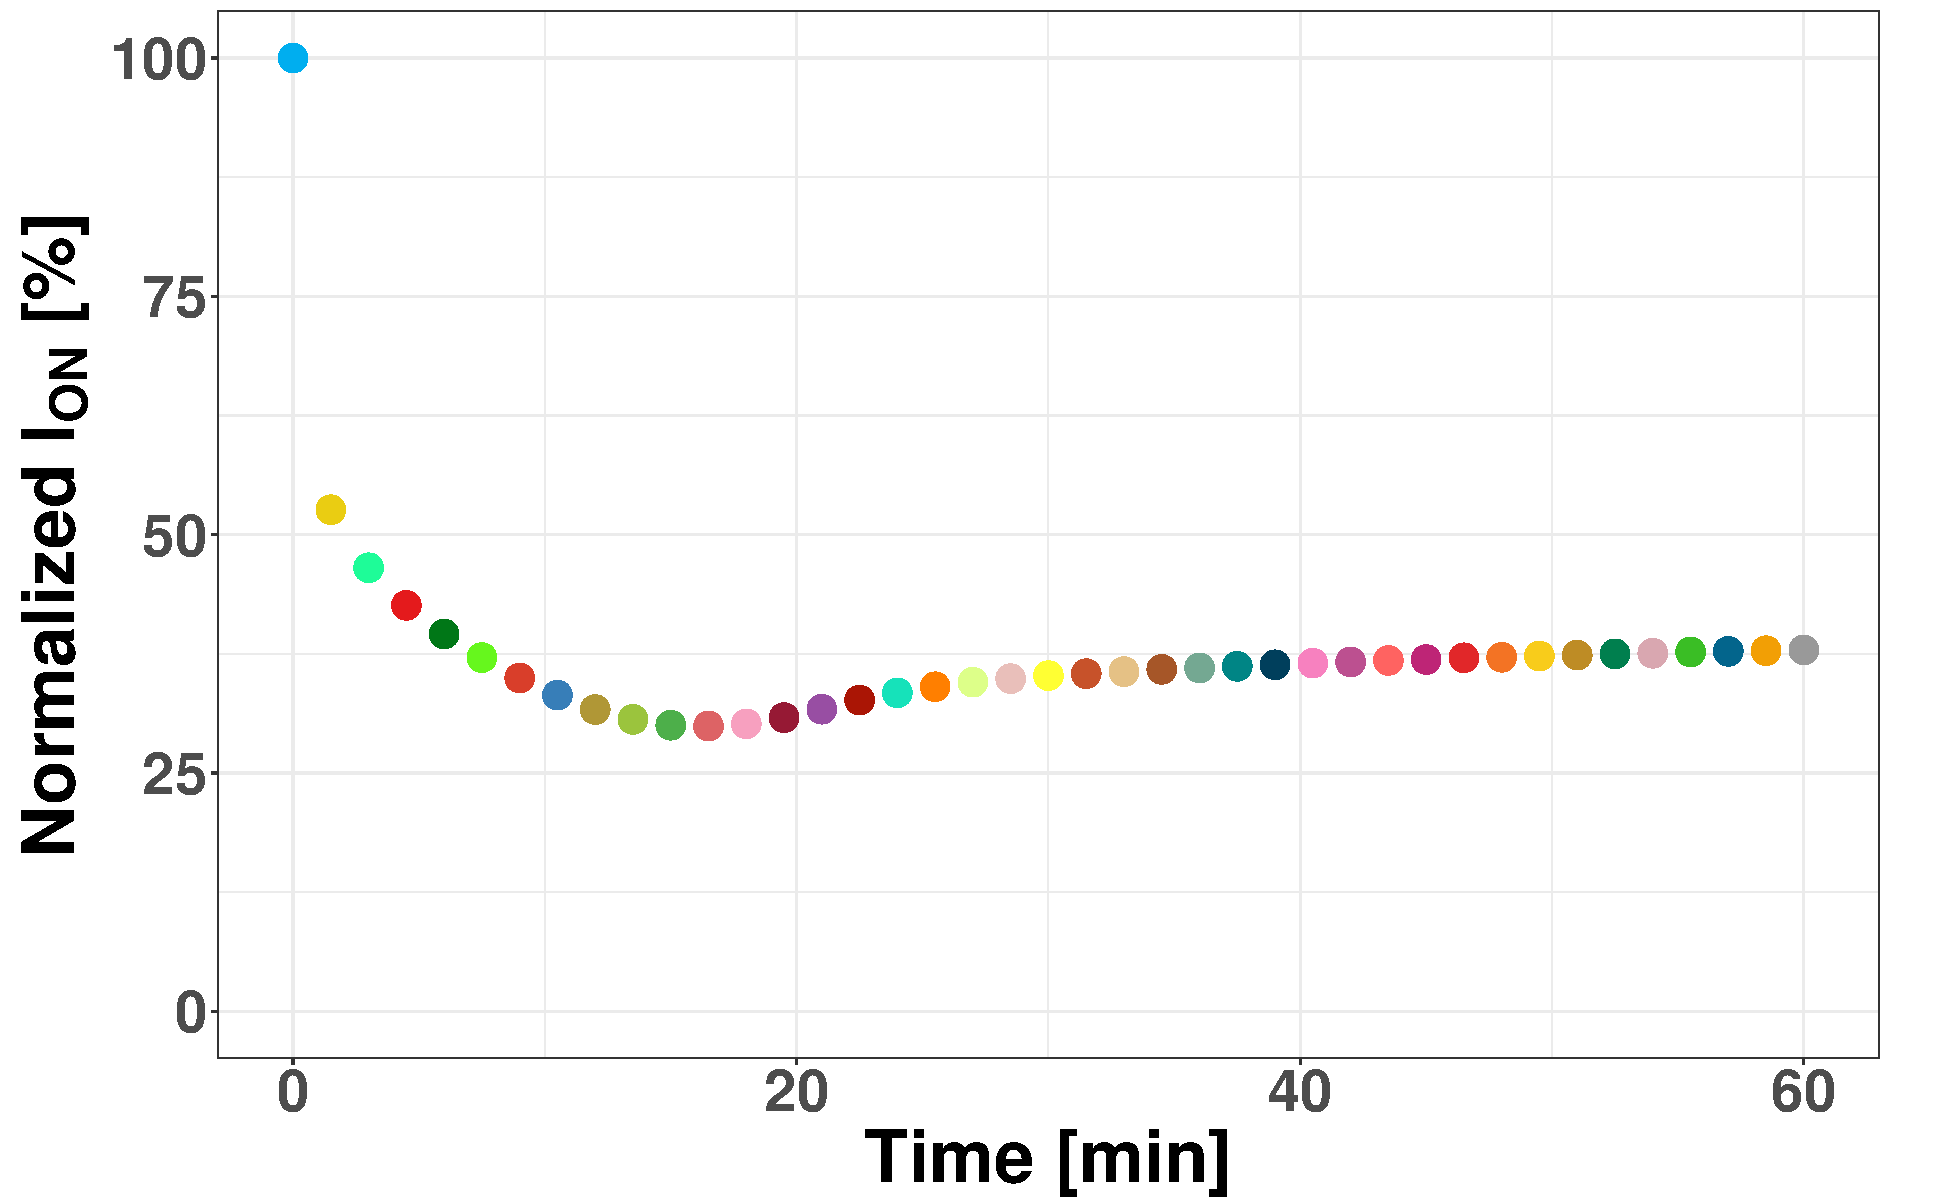
\includegraphics[width = 0.45\textwidth]{figures/chapter3/nEGFET/nNormalized_up.pdf}
        \label{fig:nNormalizedUp}
    }
    \caption{Electrical characterization of two nEG-FET devices. 
    (a) and (b) show the transfer curves and normalized current for a device that failed to stabilize, respectively. In this device, the current continuously decreases over time.
    (c) and (d) display the transfer curves and normalized current for a device that finds stabilization, respectively. This behaviour mirrors what has been observed before for the encapsulated standard EG-CNTFET and the sdEG-FET, \ie{} there is a \emph{stabilization phase} first, followed by a \emph{constant slope phase} where the current increases linearly over time.
    }
    \label{fig:nEGFETData}
\end{figure}

The performance of the devices and their stabilizing capabilities were assessed as before, through the collection of transfer and output characteristics, the extraction of \ion{} and the calculation of ON/OFF ratio and \vth{}. 

Figure \ref{fig:nEGFETData} displays the transfer characteristics and the normalized current for two representative devices, showing how nEG-FETs only found stability in \SI{50}{\%} of cases, which is insufficient for reliable, consistent sensing performance. Figures \ref{fig:nTransferDown} and \ref{fig:nNormalizedDown} show a device that failed to stabilize, with a worse performance than the standard EG-CNTFET, exhibiting much lower current values that continued to worsen over time. The second device, shown through Figures \ref{fig:nTransferUp} and \ref{fig:nNormalizedUp}, did find a level of stability, as a \emph{constant slope phase} with increasing current is visible. Another important issue that does not have to be overlooked is the fact that when these devices did stabilize, they did so with great variability, as stabilization occurred on average at \SI{25.25}{\pm 11.32}{min}. Despite all this, a full characterization of the devices was performed to gain more insight into the performance of nEG-FETs.

\begin{figure}
    \centering
    \subfloat[\ids{} and \igs{}]{
        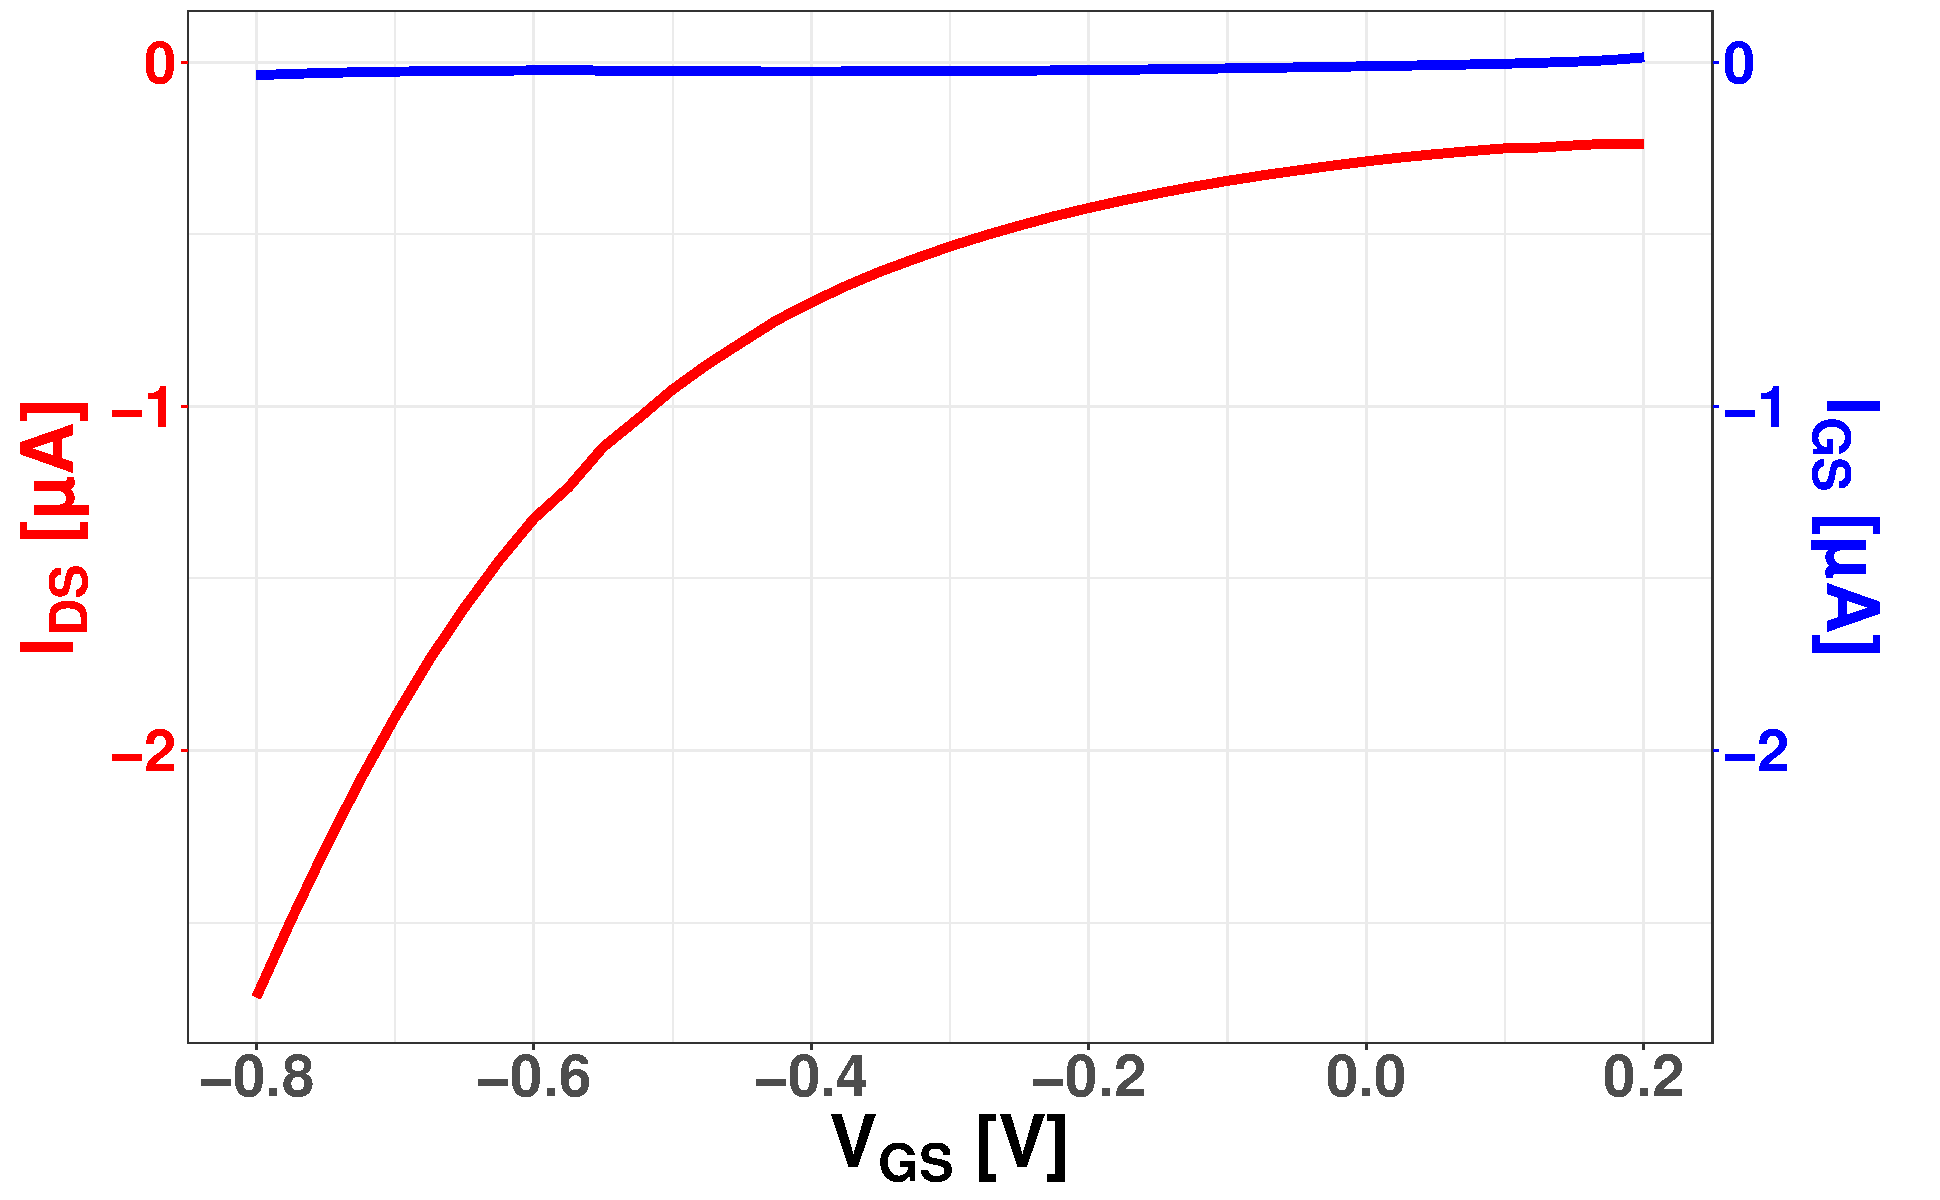
\includegraphics[width = 0.45\textwidth]{figures/chapter3/nEGFET/nIdIgCurves.pdf}
        \label{fig:nIdIgCurves}
    }
    \hfill
    \subfloat[Hysteresis]{
        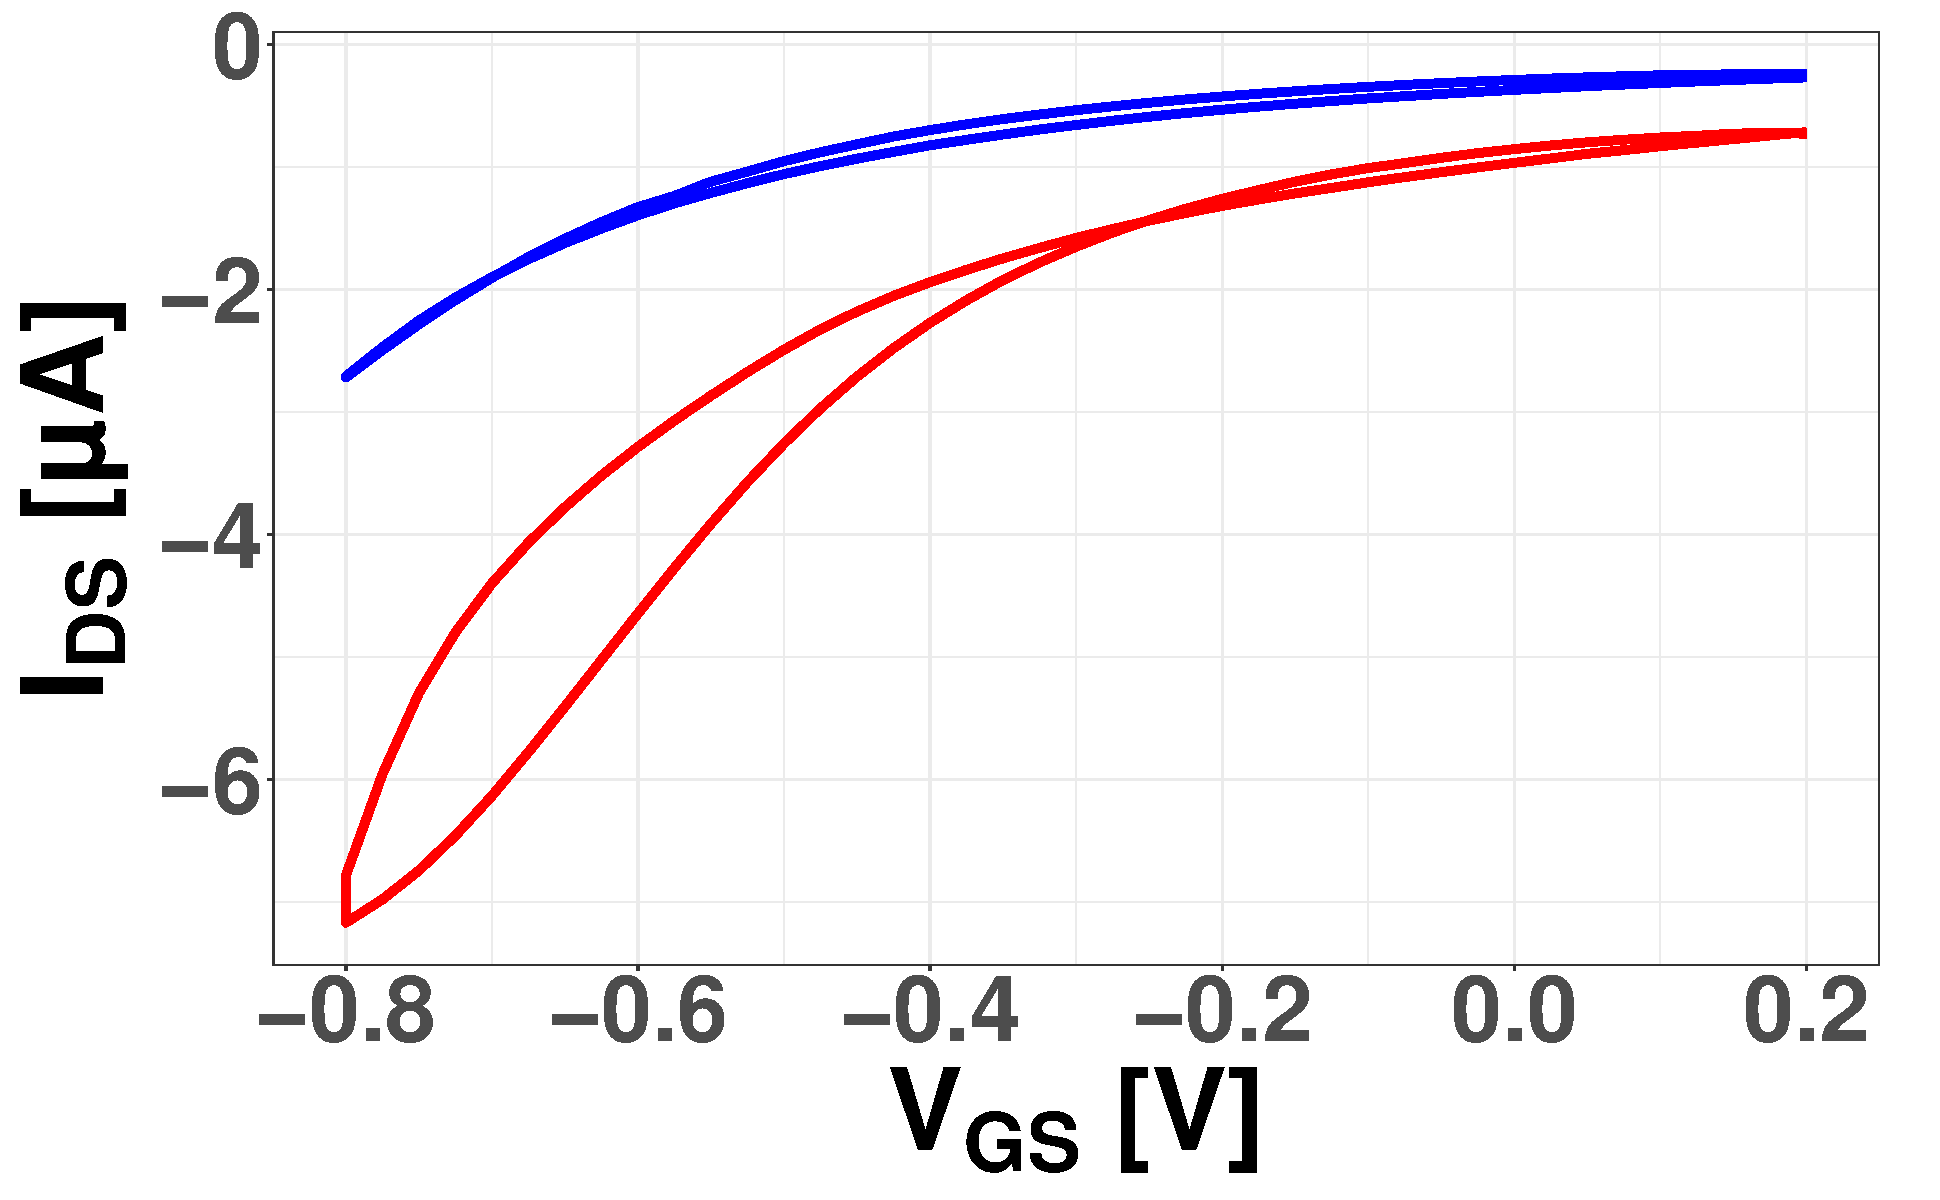
\includegraphics[width = 0.45\textwidth]{figures/chapter3/nEGFET/nHysteresis.pdf}
        \label{fig:nHysteresis}
    }
    \caption{Further electrical characterization of an nEG-FET device 
    (a) The plot shows \ids and \igs, displaying results that are comparable to those observed in the previously tested devices, where the magnitude of the \igs{} indicates minimal gate current leakage.
    (b) The hysteresis plot also demonstrates similar behavior to other devices, where it appears large at the beginning of the transfer collection, then reducing to \SI{0}{\V} at the end.}
    \label{fig:nParameters}
\end{figure}

Subsequently, to be consistent with the previous analyses, the gate current leakage and hysteresis were evaluated. The plots in Figure \ref{fig:nParameters} show that these parameters follow trends similar to those observed for the previous geometries. Indeed, the \igs{} (Figure \ref{fig:nIdIgCurves}) is orders of magnitude lower, confirming the expected behavior of the devices. The hysteresis (Figure \ref{fig:nHysteresis}) also follows a similar pattern: it starts out large for the first recorded curve, reaching \SI{0}{\V} by the end of the collection of transfer curves.

\begin{figure}
    \centering
    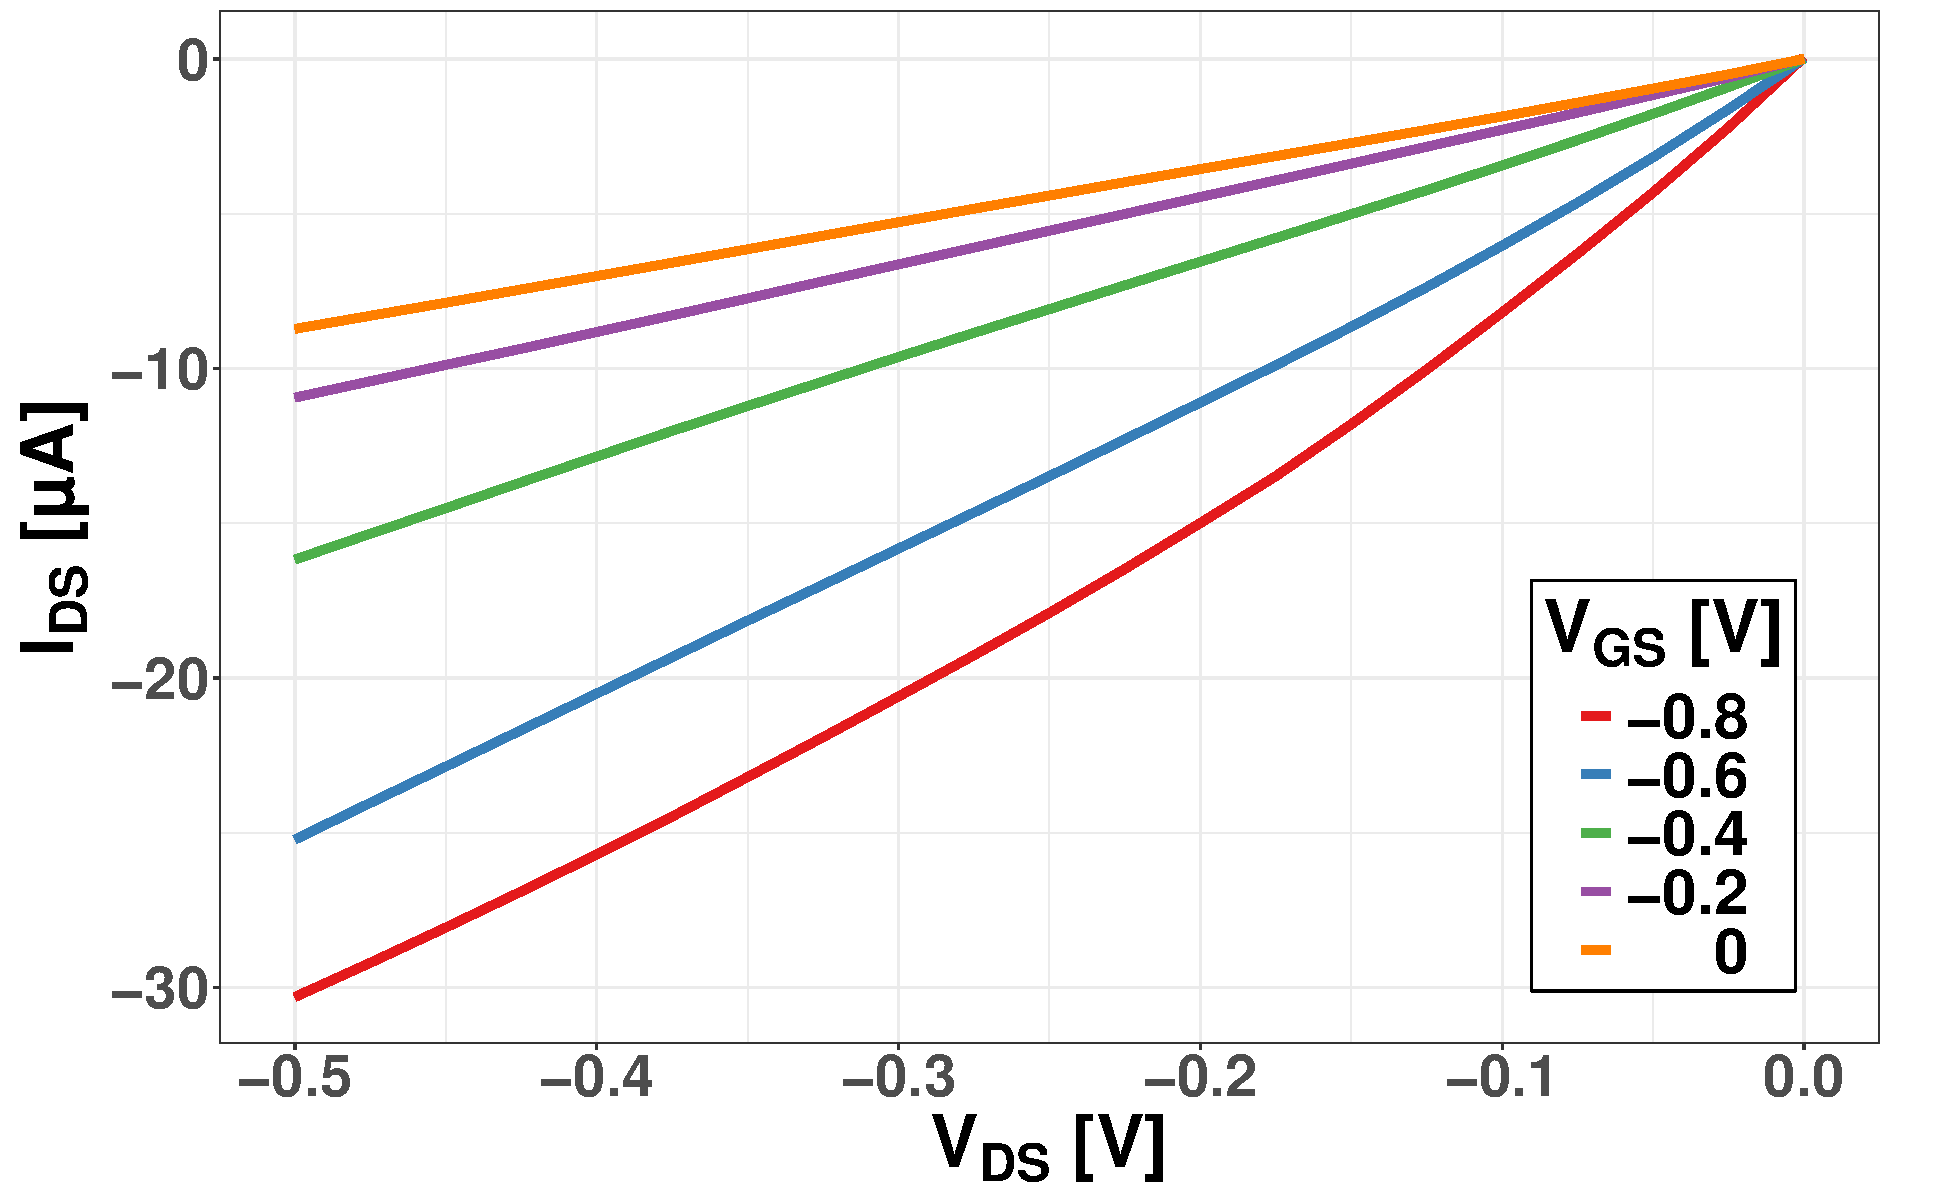
\includegraphics[width = 0.45\textwidth]{figures/chapter3/nEGFET/nOutput.pdf}
    \caption{Output characteristics of the nEG-FET. As with other devices tested, the device does not reach the saturation regime, as evidenced by the straight-line behavior observed in the output curves. This suggests that the device operates in the linear regime, which could be due to insufficient biasing or limitations in the channel length that prevent the device from achieving saturation.}
    \label{fig:nOutput}
\end{figure}

Additional measurements included the collection of the output characteristics:

\begin{figure}
    \centering
    \subfloat[On/Off ratio]{
        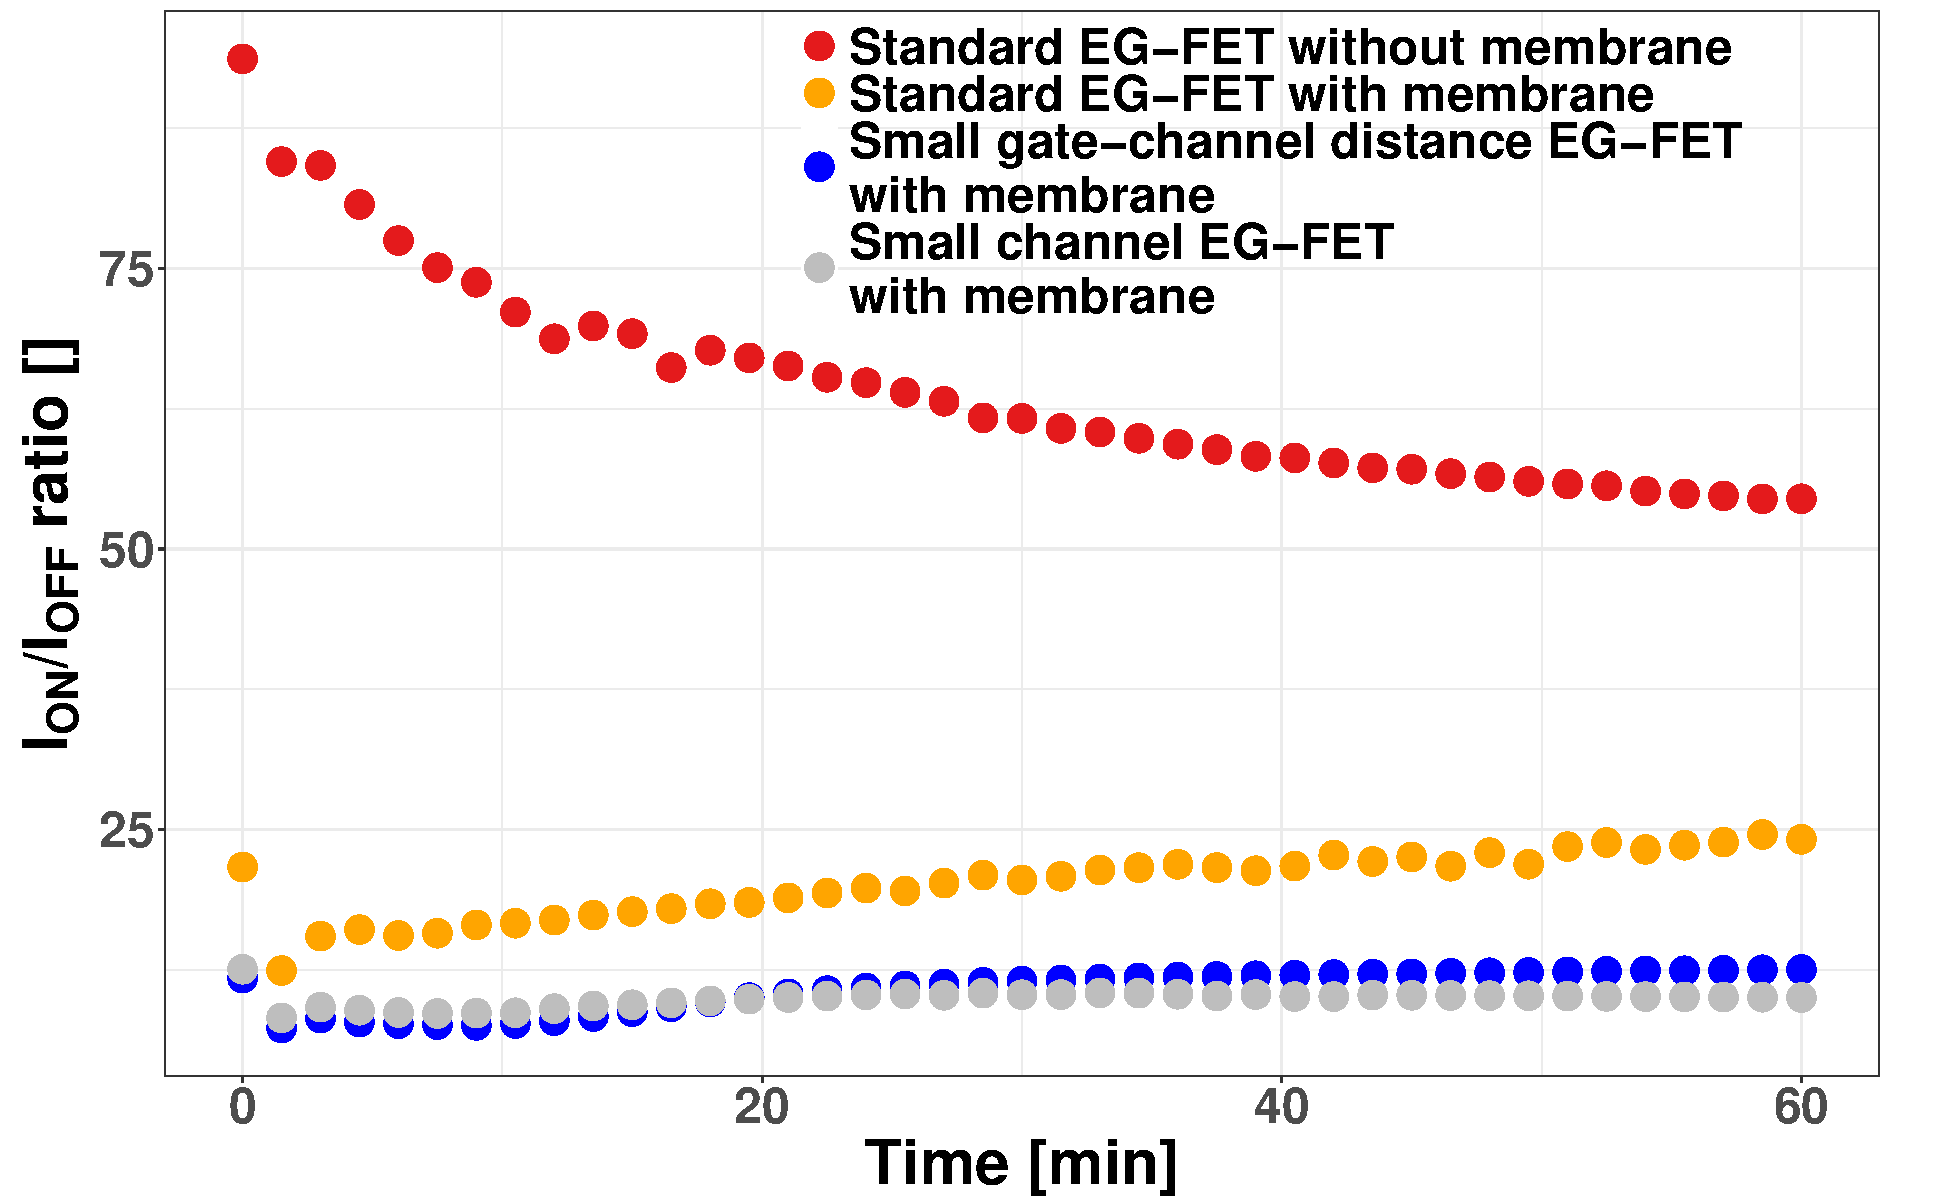
\includegraphics[width = 0.45\textwidth]{figures/chapter3/nEGFET/nOnOffRatio.pdf}
        \label{fig:nOnOffRatio}
    }
    \hfill
    \subfloat[Threshold voltage (\vth{})]{
        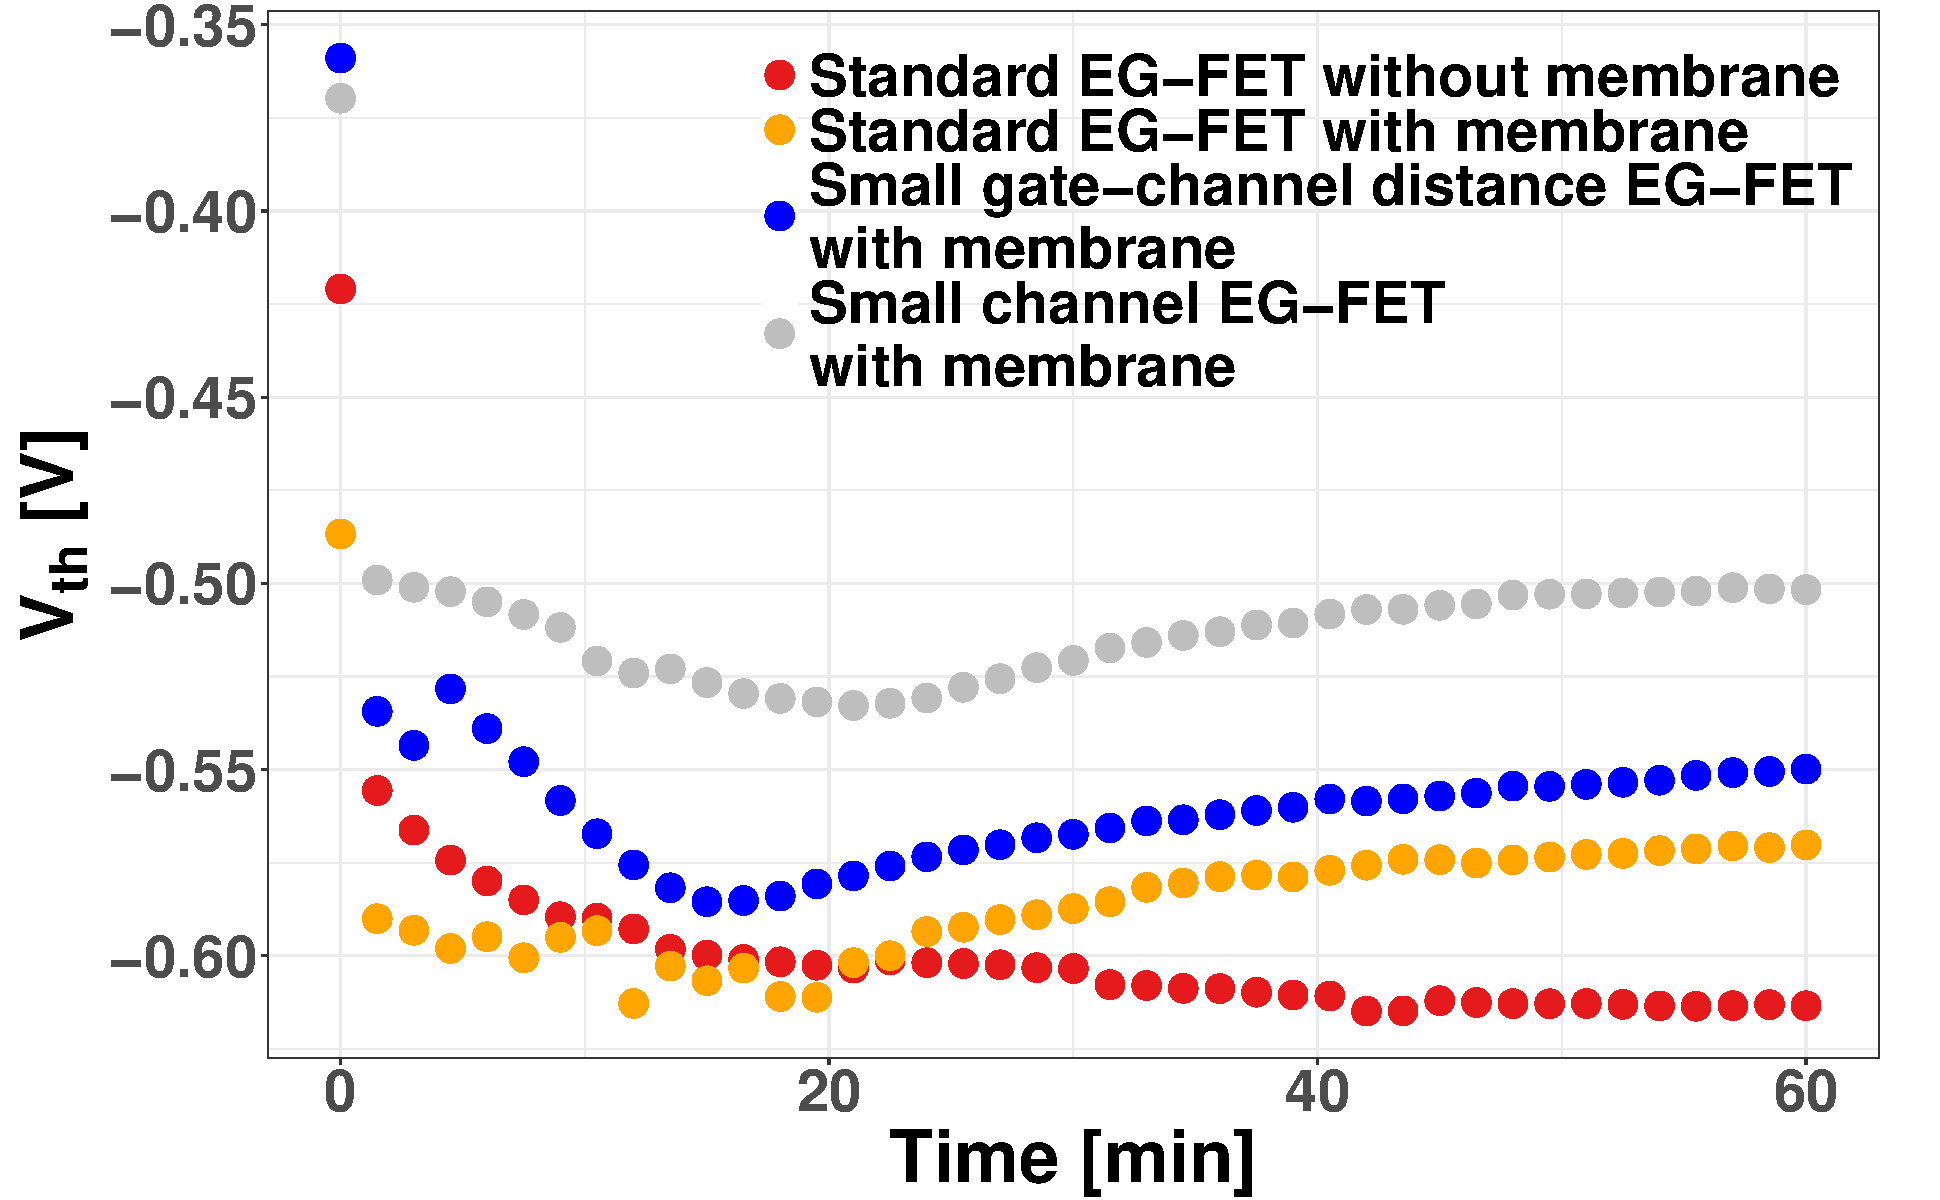
\includegraphics[width = 0.45\textwidth]{figures/chapter3/nEGFET/nVth.pdf}
        \label{fig:nVth}
    }
    \caption{Variation of (a) On/Off ratio and (b) threshold voltage (\vth{}) for nEG-FETs over time. Both plots compare the performance of the nEG-FETs with the previously analyzed geometries: the On/Off ratio is the worst among all, indicating a lower performance in terms of switching capabilities. On the other hand, the \vth{} is the smallest across all devices, suggesting that the nEG-FET requires less power to turn on, which can be beneficial for lower power consumption.}
    \label{fig:avgNParams}
\end{figure}


The performance of the nEG-FET devices, as analyzed through the on/off ratio and \vth{} in Figure \ref{fig:avgNParams}, presents mixed results. The on/off ratio is the worst among all tested devices, indicating poor switching performance. A possible explanation for this could be the reduced number of CNTs in the channel, leading to a lower overall current and a less distinct off-state. Additionally, with fewer CNTs, percolation pathways may be less efficient, resulting in increased leakage or incomplete channel modulation. On the other hand, the threshold voltage (\vth{}) is the lowest among all tested geometries, meaning that less power is required to turn on the device. This makes sense considering the smaller number of CNTs, as a lower carrier density could lead to a reduced turn-on voltage. Moreover, the smaller device area might contribute to reduced charge trapping effects, further lowering \vth{}. While this lower \vth{} could be seen as an advantage in terms of power efficiency, the overall poor performance of the on/off ratio suggests that this geometry is not ideal for sensor applications.
